\section{\pyt}
This section contains a description of how to use \pyt{}.
\pyt{} is a command line tool which requires one argument the path of the file that should be analysed and several optional arguments.
These are described below.
Alongside the description a table that shows a quick overview of the arguments can be found on \cref{pyt:arguments_overview}.

\newcommand{\pytarg}[2]{
  \texttt{#1} & #2.
}
\begin{figure}
  \begin{tabular}{l | l}
    \textbf{Argument} & \textbf{Description} \\
    \hline
    \pytarg{filepath}{Specify path of file to analyse} \\
    \pytarg{-pr, --project-root}{Specify project root} \\
    \pytarg{-d, --draw-cfg}{Draw CFG and output as a PDF file} \\
    \pytarg{-o, --output-filename}{Name of the file that is output} \\
    \pytarg{-p, --print}{Prints a CFG with simple information about the nodes} \\
    \pytarg{-vp, --verbose-print}{Same as print but with all information about the nodes} \\
    \pytarg{-t, --trigger-word-file}{Specify a trigger word file} \\
    \pytarg{-l, --log-level}{Set a log level} \\
    \pytarg{-a, --adaptor}{Chose an adaptor} \\
    \pytarg{-db, --create-database}{Create a sql file of the CFG} \\
    
\end{tabular}
  \centering
  \caption{\pyt{}s arguments.}
  \label{pyt:arguments_overview}
\end{figure}


\subsection{Positional Arguments}
As mentioned earlier \pyt{} requires one positional argument, \texttt{filepath}, which is the path of the file which should be analysed.
If the file is a part of a project the folder in which the file is in is used as root.
To specify another root one can use the optional argument \texttt{--project-root} explained below in \cref{pyt:optional}.

\subsection{Optional Arguments}\label{pyt:optional}
This section contains a brief description of the optional arguments of \pyt{}.
\todo{Tjek at den er liste passer med den endelige udgave af pyt.}

\paragraph{Project Root}
The project root argument is used for specifying the root of the project when the filepath given is not in the root folder of the project.

\paragraph{Draw CFG}
This argument is useful to visualise a CFG.
It outputs a PDF file that contains a graph like the one on \cref{theory:general_code_example_cfg}.

\paragraph{Output Filename}
This simple argument can be used to specify the output name of the file that is generated when using the \texttt{--draw-cfg} or the \texttt{--create-database} argument.

\paragraph{Print}
This outputs the CFG to the standard output in simple representation.
This prints all labels of each node in the CFG.

\paragraph{Verbose Print}
The same as the print argument but more verbose.
This means that all information a node contains is send to the output.

\paragraph{Trigger Word File}
This argument is used for specifying a trigger word file which is a file as defined in \cref{impl:vulnerabilities}.
This is optional as per default the Flask trigger word file that comes with \pyt{}.

\paragraph{Log Level}
This argument is used for setting the log level of the logger that is used.
The log level can be changed to the following level, highest level at the top:
\begin{itemize}
\item CRITICAL
\item ERROR
\item WARNING
\item INFO
\item DEBUG
\item NOTSET
\end{itemize}
The log level can be set by giving \pyt{} the following argument: \texttt{--log-level=DEBUG}.
The above will set the log level to \texttt{DEBUG}.
The default log level is \texttt{WARNING}.
By setting the log level to \texttt{CRITICAL} one will only get the loggers messages that level.
By using any level below one will get the level chosen and the ones above.
The default log level is \texttt{WARNING} and the logger writes the output of the logging to a text file ``logger.log''.

\paragraph{Adaptor}
This argument is used for specifying a framework adaptor.
Per default \pyt{} uses the Flask adaptor which comes with it, see \cref{framework_adaptor}.

\paragraph{Create Database}
\todo{write when implemented :b}

\paragraph{Help}
This options shows a short overview of the available arguments and their meaning.
On \cref{tool_overview} one can see the output when \pyt{} is run with argument \texttt{-h}.

\begin{figure}
  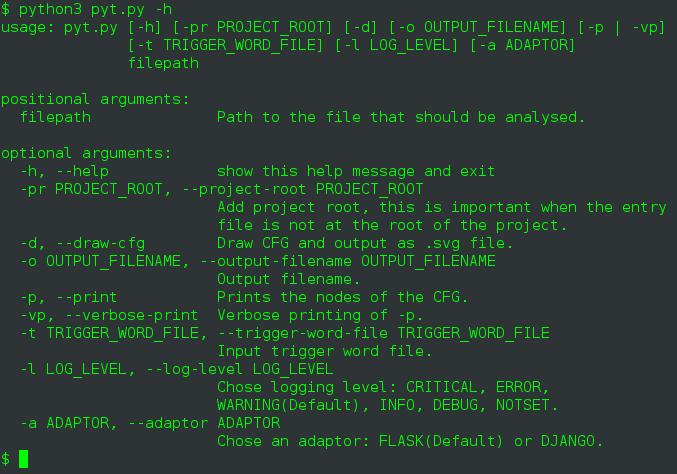
\includegraphics[width=\textwidth]{./figures/pyt_overview.png}
  \caption{An overview of \pyt{} and its arguments.}
  \label{tool_overview}
\end{figure}
